%%%%%%%%%%%%%%%%%%%%%%%%%%%%%%%%%%%%%%%%%%%%%%%%%%%%%%%%%%%%%%%%%%%%%%%%%%%%%%%
% BoletIME em LaTeX!
% O arquivo está numa folha a4 e com tamanho de fonte padrão 11pt. Não
% altere o tamanho da fonte se não quiser ter um trabalho danado!
%%%%%%%%%%%%%%%%%%%%%%%%%%%%%%%%%%%%%%
\documentclass[a4paper,11pt]{article}

%%%%%%%%%%%%%%%%%%%%%%%%%%%%%%%%%%%%%%
% Pacotes utilizados
% Para facilitar a importação centralizada de pacotes, todos os pacotes
% são importados neste arquivo de estilos. Algumas configurações da
% geometria da página, como a margem, o tamanho do cabeçalho e do rodapé
% e afins, também constam aqui.
%%%%%%%%%%%%%%%%%%%%%%%%%%%%%%%%%%%%%%
\usepackage{configs/pacotes}

%%%%%%%%%%%%%%%%%%%%%%%%%%%%%%%%%%%%%%
% Cores
% Aqui ficam as cores utilizadas globalmente, como o vermelho_camat.
% Para utilizar uma cor, basta chamar por \color{NOME_DA_COR} ou então
% \textcolor{NOME_DA_COR}{SEU TEXTO}.
%%%%%%%%%%%%%%%%%%%%%%%%%%%%%%%%%%%%%%
\usepackage{configs/cores}
% Cor do fundo
\def\corfundo{amarelo_boletime}

%%%%%%%%%%%%%%%%%%%%%%%%%%%%%%%%%%%%%%
% Fontes
% Aqui ficam todas as fontes carregadas na pasta "/fontes". Por padrão,
% são a NunitoSans Condensed, a Arimo e a ArchivoBlack.
%%%%%%%%%%%%%%%%%%%%%%%%%%%%%%%%%%%%%%
\usepackage{configs/fontes}

%%%%%%%%%%%%%%%%%%%%%%%%%%%%%%%%%%%%%%
% Meta-dados
% Configurações informadas para a edição específica, como a cor da página,
% a edição, o mês etc.
%%%%%%%%%%%%%%%%%%%%%%%%%%%%%%%%%%%%%%
%%%%%%%%%%%%%%%%%%%%%%%%%%%%%%%%%%%%%%%%%%%%%%%%%%%%%%%%%%%%%%%%%%%%%%%%%%%%
% Arquivo de configurações de edição
% Este arquivo deve ser editado conforme a edição do BoletIME.
%%%%%%%%%%%%%%%%%%%%%%%%%%%%%%%%%%%%%%%%%%%%%%%%%%%%%%%%%%%%%%%%%%%%%%%%%%%%
% Número da edição
\def\edicao{11}

% Mês e ano da edição
\def\mes{maio}
\def\ano{2024}

%%%%%%%%%%%%%%%%%%%%%%%%%%%%%%%%%%%%%%
% Helpers
% Facilitadores para processos repetivivos.
%%%%%%%%%%%%%%%%%%%%%%%%%%%%%%%%%%%%%%
\usepackage{configs/helpers}

%%%%%%%%%%%%%%%%%%%%%%%%%%%%%%%%%%%%%%
% Configurações
% Aqui ficam todas as outras estilizações e configurações do arquivo.
%%%%%%%%%%%%%%%%%%%%%%%%%%%%%%%%%%%%%%
\usepackage{configs/principal}

%%%%%%%%%%%%%%%%%%%%%%%%%%%%%%%%%%%%%%%%%%%%%%%%%%%%%%%%%%%%%%%%%%%%%%%%%%%%%%%
% Início do documento
% Tudo o que vem abaixo aparece no PDF final, até o \end{document}. A estrutura
% do documento começa pela capa, que contém a primeira página com sumário e tal,
% e vai para os textos.
%%%%%%%%%%%%%%%%%%%%%%%%%%%%%%%%%%%%%%
\begin{document}

%%%%%%%%%%%%%%%%%%%%%%%%%%%%%%%%%%%%%%
% Capa
% Neste arquivo é feita a primeira página do documento. Não é necessário alterar
% este arquivo, mas ele chama o arquivo "/sumario.tex". Este precisa ser editado
% para mostrar os títulos, resumos e páginas, além de possíveis divulgações.
%%%%%%%%%%%%%%%%%%%%%%%%%%%%%%%%%%%%%%
%%%%%%%%%%%%%%%%%%%%%%%%%%%%%%%%%%%%%%%%%%%%%%%%%%%%%%%%%%%%%%%%%%%%%%%%%%%%
% Capa
% Este arquivo gera a primeira página do BoletIME.
% No geral, não é necessário editá-lo. Para configurar os textos da primeira
% página, vá ao arquivo "/sumario.tex".
%%%%%%%%%%%%%%%%%%%%%%%%%%%%%%%%%%%%%%%%%%%%%%%%%%%%%%%%%%%%%%%%%%%%%%%%%%%%

%%%%%%%%%%%%%%%%%%%%%%%%%%%%%%%%%%%%%%
% Fundo com a imagem (cabeçalho
%%%%%%%%%%%%%%%%%%%%%%%%%%%%%%%%%%%%%%
\begin{textblock*}{\paperwidth}(0cm,0.4cm)
    \centering
    
\includegraphics[width=0.95\paperwidth]{img/boletime_cabecalho.png}\\
\end{textblock*}

%%%%%%%%%%%%%%%%%%%%%%%%%%%%%%%%%%%%%%
% Texto e linha vermelha
%%%%%%%%%%%%%%%%%%%%%%%%%%%%%%%%%%%%%%
\begin{textblock*}{\paperwidth}(0.5cm,0.275\paperheight)
    \textls[85]{
    \sffamily\bfseries
        produção do centro acadêmico da matemática, estatística e computação 
    \hspace{0.3cm} \textbar{} \hspace{1.1cm}
    \MakeLowercase{\mes}.\ano}\\    
    \textcolor{vermelho_camat}{\rule{0.95\paperwidth}{0.25cm}} % Largura e espessura do risco
\end{textblock*}

%%%%%%%%%%%%%%%%%%%%%%%%%%%%%%%%%%%%%%
% Texto no canto superior direito (nº edicao)
%%%%%%%%%%%%%%%%%%%%%%%%%%%%%%%%%%%%%%
\begin{textblock*}{5cm}(15cm, 1cm)
    \raggedleft 
    {\huge \archivoblack {nº \edicao}}
\end{textblock*}

% Espaçamento
\vspace*{0.2\paperheight}

%%%%%%%%%%%%%%%%%%%%%%%%%%%%%%%%%%%%%%
% Sumário
%%%%%%%%%%%%%%%%%%%%%%%%%%%%%%%%%%%%%%
\begin{multicols}{2}
    %%%%%%%%%%%%%%%%%%%%%%%%%%%%%%%%%%%%%%%%%%%%%%%%%%%%%%%%%%%%%%%%%%%%%%%%%%%%
% Sumário (1ª página)
% Este arquivo contém os textos exibidos na primeira página. Edite-o conforme
% for necessário. Por padrão, a seção é dividida em duas colunas, e estas não
% dividem o texto automaticamente entre si, então é necessário definir
% explicitamente o que está em cada coluna.
%%%%%%%%%%%%%%%%%%%%%%%%%%%%%%%%%%%%%%%%%%%%%%%%%%%%%%%%%%%%%%%%%%%%%%%%%%%%

% Tamanho da fonte. Pitititica
\footnotesize

\noindent\begin{minipage}[t][0.20\paperheight][t]{\columnwidth}
%%%%%%%%%%%%%%%%%%%%%%%%%%%%%%%%%%%%%%%%%%%%%%%%%%%%%%%%%%%%%%%%%%%%%%%%%%%%
%%% > O TEXTO DA PRIMEIRA COLUNA VAI AQUI
%%%%%%%%%%%%%%%%%%%%%%%%%%%%%%%%%%%%%%%%%%%%%%%%%%%%%%%%%%%%%%%%%%%%%%%%%%%%

\itemSumario{Falta de água no IME}{
Envio de um convite para refletir sobre as diferentes realidades presentes
no IME na forma de um relato sobre como é estudar de dia e de noite.
}{2}

\itemSumario{Duchamp e Tarsila}{
Uma respota ao “Mas isto até eu faço!” da edição 10 do BoletIME.
}{3}


\itemSumario{Sessão Poesias}{
Poesia encontrada na parede do banheiro da sede do DCE Livre da USP.
}{4}


\itemSumario{Sobre carta da Comissão de Recepção}{
Crítica enviada sobre a maneira como o tema da Comissão de Recepção 2024 foi conduzida.
}{5}


\itemSumario{Novo projeto acadêmico para o próximo ciclo}{
Um convite para entender o que é um projeto acadêmico, onde o IME se encontra nisso, e como a comunidade como um todo pode e deve participar da sua construção. Foi marcada a 1ª reunião aberta do projeto acadêmico para 06 de junho, às 17h no saguão do Bloco B.
}{7}

%%%%%%%%%%%%%%%%%%%%%%%%%%%%%%%%%%%%%%%%%%%%%%%%%%%%%%%%%%%%%%%%%%%%%%%%%%%%
%%% > O TEXTO DA PRIMEIRA COLUNA TERMINA AQUI
%%%%%%%%%%%%%%%%%%%%%%%%%%%%%%%%%%%%%%%%%%%%%%%%%%%%%%%%%%%%%%%%%%%%%%%%%%%%
\end{minipage}

\columnbreak

\noindent\begin{minipage}[t][0.20\paperheight][t]{\columnwidth}
%%%%%%%%%%%%%%%%%%%%%%%%%%%%%%%%%%%%%%%%%%%%%%%%%%%%%%%%%%%%%%%%%%%%%%%%%%%%
%%% > O TEXTO DA SEGUNDA COLUNA VAI AQUI
%%%%%%%%%%%%%%%%%%%%%%%%%%%%%%%%%%%%%%%%%%%%%%%%%%%%%%%%%%%%%%%%%%%%%%%%%%%%

\itemSumario{DCE Livre da USP: chapa Fazer Valer a Luta eleita para o mandato 2024/2025}{
Confira os resultados e estatísticas das eleições do DCE Livre da USP 2024.
}{8}

\itemSumario{Efeito da redução da jornada sobre os salários}{
Trecho do segundo capítulo do livro Salário, preço e lucro, de Karl Marx.
}{9}

\vspace{1cm}

\quadradao{\LARGE}
{1.4}
{50}
{.9\textwidth}
{vermelho_camat}
{0.2cm}{
- É pavê ou pacumê?\\
- Sim.}

% gorrinho natalinho no bloco
\begin{textblock*}{5cm}(18cm, 15.3cm)
    
\includegraphics[width=0.5\linewidth]{textos//img/gorro.png}
\end{textblock*}

%%%%%%%%%%%%%%%%%%%%%%%%%%%%%%%%%%%%%%%%%%%%%%%%%%%%%%%%%%%%%%%%%%%%%%%%%%%%
%%% > O TEXTO DA SEGUNDA COLUNA TERMINA AQUI
%%%%%%%%%%%%%%%%%%%%%%%%%%%%%%%%%%%%%%%%%%%%%%%%%%%%%%%%%%%%%%%%%%%%%%%%%%%%
\end{minipage}
\end{multicols}

%%%%%%%%%%%%%%%%%%%%%%%%%%%%%%%%%%%%%%
% Imagem de divulgação do BoletIME
%%%%%%%%%%%%%%%%%%%%%%%%%%%%%%%%%%%%%%
\begin{textblock*}{\paperwidth}(0cm, 0.82\paperheight)
    \centering
    
\includegraphics[width=0.95\paperwidth]{img/qr_code.png}
\end{textblock*}
\pagebreak

%%%%%%%%%%%%%%%%%%%%%%%%%%%%%%%%%%%%%%
% Conteúdo
% Tudo o que vem abaixo é o conteúdo do BoletIME. Por padrão, as páginas são
% divididas em duas colunas, que separam o texto automaticamente. Caso desejado
% seguir outro formato, consulte a documentação do pacote MULTICOLS.
%%%%%%%%%%%%%%%%%%%%%%%%%%%%%%%%%%%%%%
% estilo com cabeçalho
\pagestyle{fancy}
% espaço entre as linhas
\linespread{1.2}\normalsize
% textos
%%%%%%%%%%%%%%%%%%%%%%%%%%%%%%%%%%%%%%%%%%%%%%%%%%%%%%%%%%%%%%%%%%%%%%%%%%%%
% Conteúdo do BoletIME
% Aqui ficam os textos e todo o conteúdo do BoletIME a partir da segunda
% página.
%%%%%%%%%%%%%%%%%%%%%%%%%%%%%%%%%%%%%%%%%%%%%%%%%%%%%%%%%%%%%%%%%%%%%%%%%%%%

%%%%%%%%%%%%%%%%%%%%%%%%%%%%%%%%%%%%%%
% Isso quebra a página em duas colunas
%%%%%%%%%%%%%%%%%%%%%%%%%%%%%%%%%%%%%%
\begin{multicols*}{2}

% "FALTA DE ÁGUA NO IME", por anonimo
% texto enviado pelo forms
\section*{Falta de água no IME}
\autoria{anônimo}
\avisoTextoForms

Desde o ano de ingresso, sempre estudei de manhã como estudante do diurno. Neste último semestre, por conta de forças maiores e circunstâncias de vida, acabei tendo que pegar matérias de noite. Além do horário de aulas e horas de sono, muitas outras coisas que nunca imaginei ser o caso mudaram também. O transporte público na ida deixou de ser a superlotação das 6 da manhã. Em compensação, no entanto, o transporte de volta virou uma corrida contra o tempo, uma vez que o metrô fecha meia-noite - e a escassez de Circulares durante o período noturno não ajuda -. A disposição para fazer qualquer atividade durante a semana mudou, já que agora parece que meus dias não rendem tanto pela perda do período de tarde livre. Estar em uma sala de aula com pessoas novas e que nunca vi na vida também foi algo que, mesmo tendo a ciência de que aconteceria, foi um pequeno choque de qualquer forma.

Houveram muitos dias em que fui olhar o cardápio dos bandejões de almoço ao invés do jantar. Mas mesmo quando lendo o cardápio certo, às vezes simplesmente não conseguia chegar a tempo de comer e assistir às aulas, e o fechamento da lanchonete às 21h faz com que não seja possível comer algo durante a troca de aulas no mesmo horário. Sobre isso, algo que tem ajudado muito, nesse sentido, foi o CAMat ter ampliado sua gama de alimentos para venda.

A inspiração para a escrita desse texto, no entanto, veio após ter saído da aula numa sexta-feira, ido ao banheiro, e perceber que não tinha água na torneira para lavar as mãos. Passei em todos os banheiros, e o mesmo se repetiu em todas as pias de todos os banheiros do Bloco B. No fim, consegui lavar as mãos somente no banheiro do Bloco A. Como nunca tinha acontecido isso comigo, fui conversar com meus veteranos sobre, mas ninguém pareceu surpreso com o fato, e pareceu ser algo que simplesmente acontece.

Por curiosidade, fui atrás para tentar entender melhor a situação, e descobri que, não só como é um problema que existe desde muito antes do meu ingresso, como também é um problema conhecido, como mostra o repasse abaixo datada de 2020, encontrado no Telegram do CAMat:

“A falta de água, no período noturno, nos bebedouros do bloco B é um problema que se fez recorrente nos últimos semestres e o qual não obtínhamos quaisquer explicação por parte da diretoria do IME. Contudo, no último Conselho Técnico Administrativo (05/03), foi informado que a origem da falta de água é a SABESP, que diminui a pressão à noite, e que a equipe de manutenção do IME já está buscando resolver o problema - seja diretamente com a SABESP ou internamente. Além disso, foi pontuado que ainda nesse ano (2020) será instalada uma caixa d’água no bloco B - requerimento do corpo de bombeiros -, o que ajudará a solucionar o problema.”

\begin{figure}[H]
    \centering
    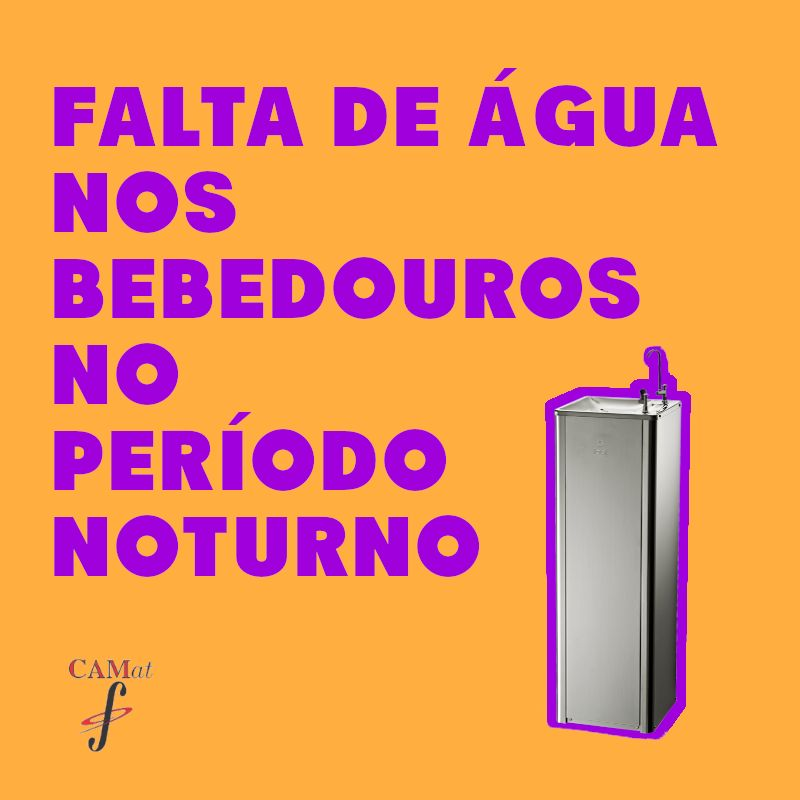
\includegraphics[width=0.65\linewidth]{textos/img/post_telegram_camat.jpg}
    \\
    \legendaFigura{1}{\textit{post do telegram} \legendaFiguraQuebraLinha Acervo CAMat}
    \vspace{-0.5cm}
\end{figure}

Quando converso esporadicamente com meus amigos do diurno - e que continuaram no diurno -, nenhuma dessas questões parecem ser evidentes para eles, do mesmo jeito que não foi evidente para mim antes de eu ter tido a necessidade de vir para noturno. Grande parte dessa separação, ao meu ver, se dá pela distância que existe entre as turmas do diurno e noturno. Não existe um diálogo muito forte entre as duas. São pessoas que vivem em realidades diferentes com necessidades diferentes. Como exemplo disso, lembro que na minha sala do diurno, poucos trabalhavam, ao ponto que na minha sala do noturno, trabalhar e depois vir para aula parece ser a regra. Isso, claro, não é uma crítica ao diurno, tampouco estou colocando juízo de valores. Apenas exponho que, na minha percepção, existem essas realidades diferentes, e que acredito ser importante para que, enquanto imeanos, entendermos a existência das outras realidades dos ambientes que frequentamos.

\pagebreak

% "DUCHAMP E TARSILA", por Celestino B. Neto
% texto enviado pelo forms
\section*{Duchamp e Tarsila}
\autoria{Celestino B. Neto}
\avisoTextoForms

Li com alegria o texto apócrifo recém publicado no BOLETIME, onde um anônimo especula sobre a ideia de um parentesco entre Arte e Matemática. É importante que haja porosidade entre o universo das “humanas” e o das “exatas”.

Assim como um de nós, que estude matemática, poderia se insurgir com a afirmação de que “não existe muita diferença entre números racionais e números reais, pois ambos podem ter vírgulas seguidas de vários números”, alguém, com algum conhecimento na área de “humanas”, poderia se incomodar com generalizações, ainda que bem intencionadas, nas áreas da literatura, e das artes plásticas.

\begin{displayquote}
    \textit{\textbf{``...Malgré ses affinités avec Dada ou les surréalistes, Duchamp reste un artiste indépendant...''}}[1]
\end{displayquote}

Marcel Duchamp, artista independente, que flertou com diversos movimentos artísticos (dadaismo, fauvismo e cubismo), foi quem introduziu os “ready made” [2] no universo das artes plásticas . A “Roda de bicicleta”, criada em 1913 [3] foi sua primeira manifestação. A proposta do artista era deslocar “\textbf{objetos comuns, com ou sem modificações mínimas, para dentro de espaços museológicos}” [4], com o intento de se aproximar do conceito de indiferença visual. Isso liberaria o artista do império da “arte retiniana”, aquela voltada ao deleite visual, convidando, por outro lado, os apreciadores a uma reflexão sobre a linguagem da arte, o que abriu a via para a consolidação da ideia de arte como conceito [5].

Assim, a obra “Roda de bicicleta”, no contexto em que se inseria, não se vincula à discussão utilidade/inutilidade de um determinado objeto, como insinua o texto apócrifo publicado. Não está aí o compromisso do fazer artístico. “\textbf{Duchamp... mostrou a obra de arte pronta [6] como um subproduto, resultado de uma “digestão” artística. A partir da intervenção do artista, o objeto, agora um trabalho artístico, incorpora um valor cultural.}” [7].

\begin{figure}[H]
    \centering
    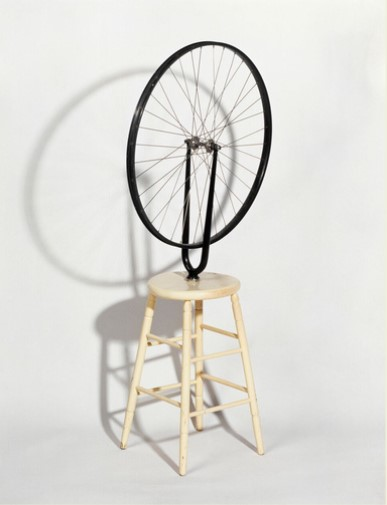
\includegraphics[width=0.65\linewidth]{textos/img/duchamp_a_roda_de_bicicleta.jpg}
    \\
    \legendaFigura{1}{\textit{A Roda de Bicicleta, Marcel Duchamp}}
\end{figure}

Já o “Abaporu”, de Tarsila do Amaral, foi concebido como presente ao seu então marido, o escritor Oswald de Andrade, que ao recebê-lo nomeou (junto ao poeta Raul Bopp) a obra à partir de vocábulos da língua tupi que significam “homem que come gente”, criando assim um vínculo com o Movimento Antropofágico “que se propunha a deglutir a cultura estrangeira e adaptá-la ao Brasil” [8].

Insinua o texto apócrifo, que Tarsila teria tido a intenção de retratar um Abaporu [9]. Sabe-se que esta obra, ícone do modernismo brasileiro, “através do emprego de cores puras, das linhas simples, da captação sintética, sentimental e ingênua da realidade brasileira” [10], nos passava uma mensagem plástica regionalista (brasileira), cujo conteúdo foi desvelado posteriormente por Oswald.

\begin{figure}[H]
    \centering
    
\includegraphics[width=0.65\linewidth]{textos/img/tarsila_abaporu.jpg}
    \\
    \legendaFigura{1}{\textit{Abaporu, de Tarsila do Amaral}}
\end{figure}

Foi feliz a escolha de Duchamp e de Tarsila no texto apócrifo, dois marcos que são na produção artística do séc.XX, assim como a tentativa de inserção de elementos não matemáticos no ambiente do IME, como forma de alargar a visão limitada do mundo que somos levados a nutrir, em função da falta de tempo que a grade curricular nos impõe. Fica então uma sugestão: mais rigor nos “axiomas” que escolhemos ao fazer a “demonstração de um teorema” não matemático, se me permitirem esta transposição.

O mesmo rigor empregado no fazer da Matemática precisa ser valorizado na produção de textos e no uso da língua, no ambiente da Matemática, para que aquilo que escrevemos tenha recepção adequada e relevante nos ambientes acadêmicos menos afeitos aos números, mas absolutamente comprometidos com o rigor das proposições.

\emph{\textbf{Sobre o autor:} Celestino Neto cursa atualmente, no IME- USP, o terceiro semestre de licenciatura em Matemática (noturno), é arquiteto formado pela FAU-USP e bacharel em Letras com habilitação em Português e Linguística pela FFLCH-USP.}

\vfill % para grudar no fim da página

\textbf{[1]} \emph{Tradução livre: “...Apesar de afinidades com Dada ou os surrealistas, Duchamp continua sendo um artista independente”}
\\
\textbf{[2]} \emph{Tradução livre: “obra de arte pronta”}
\\
\textbf{[3]} E não em 1951 como informa o texto apócrifo.
\\
\textbf{[4]} \emph{Ready Made: Inclusão Ruidosa}; PELED, Yiftah, pg. 1724
\\
\textbf{[5]} Enciclopédia Britannica para “Conceptual art”. \emph{Tradução livre: “arte conceitual tem sido descrita como um dos movimentos mais influentes do final do sécXX, uma extensão lógica do trabalho iniciado pelo artista francês Marcel Duchamp em 1914 para quebrar a primazia do perceptivo em arte.”}
\\
\textbf{[6]} “ready made”
\\
\textbf{[7]} Ready Made: Inclusão Ruidosa; PELED, Yiftah, pg. 1727
\\
\textbf{[8]} Programa de pos-graduação em artes visuais da UFBA
\\
\textbf{[9]} “O Abaporu jamais foi visto em qualquer lugar, por mais remoto que seja, mas ainda assim Tarsila do Amaral foi capaz de retratá-lo”
\\
\textbf{[10]} Abaporu e a “invenção” da arte brasileira; SILVA, Dalmo de Oliveira Souza e, pg. 540

% ENIGMA
% professor preguiçoso
\section*{Enigma do BoletIME - Resolva e ganhe 1 Trento}

A primeira e a décima pessoa a apresentarem a solução correta do enigma abaixo para o CAMat (seja pelo envio no e-mail ou pessoalmente para algum membro da gestão) ganhará um Trento da lojinha do CAMat. Boa sorte!

Um professor do IME decidiu, após 4 anos lecionando, contabilizar quantas avaliações corrigira. O professor deu aula em todos os períodos para apenas uma turma, que sempre era composta de 40 alunos. Para avaliar seus estudantes, ele aplicou 2 provas durante o semestre, não ofereceu substitutivas e tem um sistema de atividades para que a pessoa escolha, dentre as quatro listas oferecidas, duas para serem feitas e corrigidas. Ele constatou que, em cada uma das suas avaliações (provas e atividades), exatamente 9 alunos estavam ausentes ou simplesmente não a entregaram. Curiosamente, o professor também sabe que apenas 9 alunos já fizeram a prova de recuperação.

O professor decidiu, então, conferir no sistema quantas avaliações haviam sido feitas, mas, infelizmente, o sistema apresentou falhas no armazenamento. Sabe-se que o sistema registra a quantidade de notas numa base 10, mas a falha acabou transformando os algarismos em letras de modo que letras iguais representam números iguais. Ademais, a falha também acabou multiplicando a quantidade de avaliações pelo número de estudantes que não compareceu às provas acrescido do dia do mês em que a consulta foi feita.

Determine uma combinação de letras que o sistema pode ter apresentado quando consultado após as falhas.

\barraVermelha % uma divisória vermelha

% SEÇÃO DE POESIAS
\tituloCaixa{SEÇÃO DE POESIAS}

\vfill % para grudar no fim da página

\emph{autor desconhecido}\\
Não tinha papel (é o banheiro do DCE)\\
e tinha uma mariposa no vaso (banheiro do DCE)\\
que eu matei sem misericórdia (me perdoa, mariposa)\\
\\
\sout{bom} boa tarde a todos

\pagebreak % quebra de página

% "SOBRE A CARTA DA COMISSÃO DE RECEPÇÃO", por anônimo
% texto enviado pelo forms
\section*{Sobre a carta da Comissão de Recepção}
\autoria{anônimo}
\avisoTextoForms

As Gincanas da Semana de Recepção do IME é um evento que ocorre todo início de ano, e sempre conta com a participação de veteranos e calouros em uma série de atividades, palestras e jogos projetadas para enturmar a calourada e fazê-la conhecer os espaços do IME e da própria USP. Organizada pela Comissão de Recepção, um tema é sempre decidido no ano anterior para o ano consequente. Em 2022, o tema escolhido foi Shrek; em 2023, foi Scooby- doo; e assim por diante. Para acomodar as temáticas escolhidas, são feitas identidades e dicas visuais usando tanto figuras em si de cada tema, como também cores que representam o tema. Além disso, as atividades programadas e todo aparato adjacente das atividades - premiação, nome da atividade, formato, etc - também acompanham a temática escolhida.

Neste ano de 2024, a Comissão acabou por optar na escolha do tema de Kung Fu Panda, aproveitando o esperado lançamento do quarto filme da franquia nos cinemas. Por se tratar de uma franquia que, de muitos modos, possibilita uma aproximação com a ideia de “Kung Fu na visão do Ocidente”, e existem nela elementos que inevitavelmente podem remeter ao senso-comum sobre o que é Kung Fu, o que é China, e principalmente no reforço de uma ideia visual de “Oriente-extremo” como um todo quando se toma uma visão descuidada na sua interpretação. Para isso, basta observar como a filosofia de Kung Fu é retratada em peças de mídia chinesa e em Kung Fu Panda.

A partir de contos, poemas e histórias dentro dos vários universos literários chineses, a ideia de Kung Fu é retratada de maneira a não glorificar violência e tecnicalidades. Kung Fu, na literatura chinesa, é interpretado como um estado de ser que foca na iluminação intelectual. A própria palavra Kung Fu no seu sentido literal não sugere estritamente luta, mas sim “fundamentos” - para qualquer coisa -. A sua tradução ao pé da letra pode ser entendida como “habilidade” ou “saber de algo”, ao ponto do termo ser usado como expressão para alguém habilidoso: “Uau! Você realmente dedicou kung fu nos estudos!”.

Em contraste, Kung Fu Panda parece inevitavelmente seguir o tropo hollywoodiana do Escolhido: um herói inserido em um mundo estranho, conhece um mentor, descobre aliados, e combate o mal. Aqui, Kung Fu é visto como um conjunto de técnicas que necessariamente existem para aperfeiçoar a fisicalidade da luta e somente: os Cinco Furiosos são reverenciados pela sua agilidade, força e ferocidade, e são de fato tratados como estrelas de filme; e o Po é visto como um instrumento para derrotar o vilão. Assim, Kung Fu Panda não é um filme sobre a China.

É nesse contexto que a Comissão de Recepção 2024 escreve no Relatório da Semana de Recepção aos Calouros enviado à pró-reitoria que “[…​] Logo após tais premiações, a equipe com a maior pontuação obtida ao longo da gincana foi premiada com macarrão instantâneo e hashi, muito comuns na culinária chinesa, fazendo assim referência a temática da semana de recepção Kung-fu Panda […​]”.

Por um, o relatório dá a entender que existe uma unicidade na culinária chinesa, que não condiz com a realidade. Hoje, são oficialmente reconhecidos pelo Estado da República Popular da China 56 do que ficou traduzido como “etnias” dentro do seu território continental, e a sua diversidade se mostra em todos os aspectos possíveis: desde cultural, religioso, fenotípico e, claro, alimentar. Enquanto que os Han fazem o consumo normal de carne suína, por exemplo, os Hui - que representam, a depender da província, até 90\% da população local - não fazem por ser uma etnia tradicionalmente islâmica-sunita. Nesse sentido, é um erro assumir que existe somente uma China, pois de fato existem várias “Chinas”, sendo esta uma análise necessária a se ter consciência.

Em segundo plano, o aspecto mais gritante ao afirmar que macarrões instantâneos são “muito comuns na culinária chinesa” é o reforço dos estereótipos construídos ao longo da história sobre aquilo que se entende por China no Brasil, agravado pela ideia do uso de Hashi. Claro que macarrões são consumidos na China, e constitui um dos pilares alimentares das várias culturas que coexistem e intersectam, e de fato utensílios parecidos com Hashi são usados. Porém, a maneira como macarrões instantâneos existem no Brasil não é um reflexo fiel do alimento consumido na China, tampouco o uso do termo Hashi demonstra uma preocupação em entender a origem do termo no contexto histórico brasileiro quanto à vinda e presença desses imigrantes. Foi ignorada, nesse aspecto, a existência de erros fundamentais de coerência histórica e linguística. O macarrão instantâneo encontrado nos mercados de hoje é uma invenção japonesa - fato verificável com uma rápida busca de 4 segundos -. O termo “Hashi”, também, é a transliteração japonesa para o utensílio. Claro que, mecanicamente, Hashi e Kuaizi são muito parecidos. Mas conceitualmente e, de certa forma, culturalmente não são, uma vez que a linguagem não é neutra. O fato do utensílio ser oficializado no Brasil como Hashi e não Kuaizi ou Jeotgarak vem de uma disputa histórica pelo domínio da narrativa sobre quem define o que é o “oriental”. Não à toa que na Zona Central de São Paulo existe a Praça da Liberdade África-Japão que, além de colocar África como em igual status de país justaposta ao Japão, faz parecer que existe uma predominância japonesa na região - o que não é verdade -.

Tudo isso e outros problemas são, em essência, frutos de uma análise inefetiva da franquia que foi usada como tema para a Semana. Assim, retoma-se a discussão sobre Kung Fu Panda não ser um filme sobre a China: a franquia nunca se propôs a ser. A construção de mundo e narrativa em Kung Fu Panda é, nas palavras do co-diretor do primeiro filme John Stevenson, “[…​] Vamos fazê-lo um filme de artes marciais de verdade, um que tenha um personagem cômico […​]”. Kung Fu Panda, em essência, é uma carta de apreciação que os produtores dedicaram aos filmes de Kung Fu - filmes estes que os próprios produtores cresceram assistindo -; e nisso, Kung Fu Panda se mostrou detalhista e respeitável quando, ao longo da franquia, são usadas de maneira respeitosa referências cinematográficas que trazem memórias do que a indústria cinematográfica de Hong Kong uma vez foi. O design de Po é, para além da quebra da ideia de que somente o mais fisicamente apto pode praticar lutas, é também uma referência ao cinema de Sammo Huang; muitas cenas fazem uma releitura de Kung-Fusão de Stephen Chow; o uso livre de objetos como parte da luta é uma referência ao humor de Jackie Chan.

Sobre isso, a Comissão cometeu um erro de leitura ao entender Kung Fu Panda como “China”, agravado pelo uso de elementos que flertam com um processo histórico de racismo. A própria fonte utilizada nas artes e postagens evocam um senso de “orientalidade” através de uma espécie de reinterpretação de traços da escrita chinesa adaptados para escrever o alfabeto latino. Dentro do design gráfico, esse tipo de fonte é chamado de “fontes wonton” ou “fontes chop-suey”, um sub-gênero da família de “fontes étnicas”, desenhadas para criar uma identidade visual que seja associada a grupos étnicos específicos: como a fonte que evoca uma ideia de “África” usada nos cartazes para O Rei Leão - O Musical. É a equivalência escrita de sotaques estereotipados, ainda mais considerando a origem indubitavelmente reducionista de fontes chop-suey e da maneira como a associação da identidade chinesa a essas fontes serviram de aparatos para terceirizar e desumanizar estes imigrantes ao longo dos séculos XVIII, XIX e XX. Nisso, vale a pena notar que Kung Fu Panda não faz o uso desse tipo de fonte em seus cartazes. 

\begin{figure}[H]
    \centering
    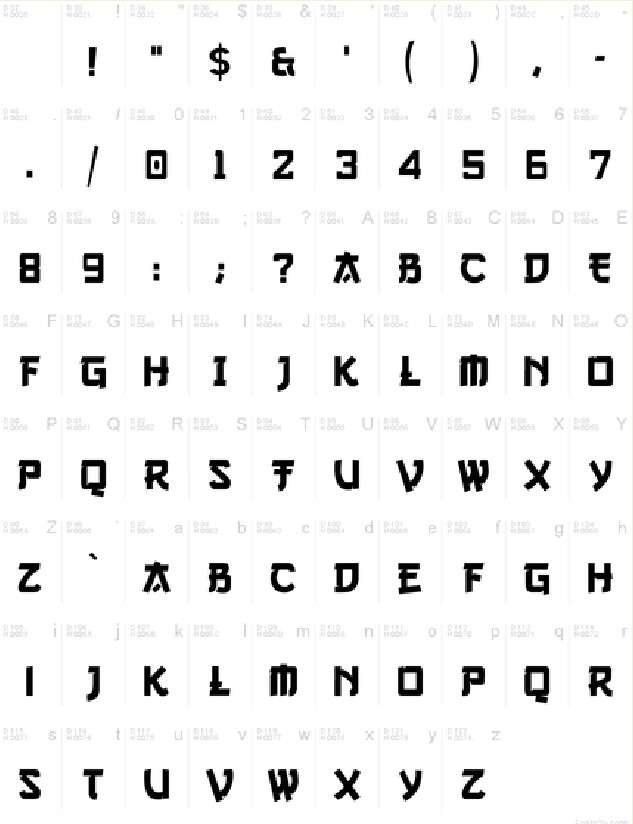
\includegraphics[width=0.7\linewidth]{textos/img/exemplo_chop_suey_gang_of_three.jpg}
    \legendaFigura{1}{\textit{"Gang of Three", exemplo de uma fonte chop-suey.}}
\end{figure}

Assim, percebe-se que, para além de ter um olhar mais sensível de entender as nuances históricas e entender que linguagem não é só o texto pleno que foi escrito, mas também a sua apresentação estética, é importante, também, fazer uma interpretação mais acurada das obras e franquias que virão a ser temas quando envolve algum elemento que não seja familiar aos membros da Comissão, seja este uma cultura nova, uma identidade nova, um visual novo; de ter a paciência de perguntar e entender: o que essa obra realmente quer dizer? 

\barraVermelha % uma divisória vermelha
\pagebreak % quebra de página

% "NOVO PROJETO ACADÊMICO PARA O PRÓXIMO CICLO"
\section*{Novo projeto acadêmico para o próximo ciclo}

O projeto acadêmico é um documento estratégico, norteando as ações do instituto e departamentos dentro de um ciclo. Como dispõe de uma análise conjuntural da unidade e estipula metas a serem alcançadas através de atitudes pontuadas como necessárias, o projeto acadêmico permite, ao final do ciclo, a realização de um balanço da atuação institucional e docente naquele período. Ou seja, este documento não é meramente técnico, mas político.

A USP está no momento de reformulação do projeto acadêmico das unidades - e o IME USP não é isolado disso. Na semana, o representante discente na Comissão de Graduação recebeu o rascunho inicial - o qual iremos disponibilizar ao lado - das metas sugeridas para o próximo ciclo de 5 anos do instituto, tendo o prazo de 9 de junho (segunda-feira) para apresentar propostas de alteração ou supressão. Posteriormente, o projeto consolidado na CG passará para a Congregação, onde novamente teremos possibilidade de intervenção.

Fazemos, então, um chamado à comunidade IMEana para realizarmos um balanço das metas postas no ciclo anterior e o quanto, na visão dos estudantes, o instituto avançou ou não. E mais, colocarmos as nossas ponderações, propostas e críticas às metas rascunhadas para o próximo ciclo. 

\quadradao{\LARGE}{1.2}{0}{\columnwidth}{black}{0.15cm}{
REUNIÃO ABERTA
\\~\\
Revisão do Projeto Acadêmico
\\~\\
06 de junho (quinta-feira) \\ às 17h | Saguão do Bloco B
\\~\\
}

% para ir para a outra coluna
\vfill\null\columnbreak

\tituloCentralizado{Formulário para Colaboração}
\begin{figure}[H]
    \centering
    
\includegraphics[width=0.5\linewidth]{textos//img/qrcode_colaboracao.png}
\end{figure}

\vspace{1cm}

\tituloCentralizado{Rascunho das metas - CG}
\begin{figure}[H]
    \centering
    
\includegraphics[width=0.5\linewidth]{textos//img/qrcode_rascunho_metas.png}
\end{figure}

\vspace{1cm}

\tituloCentralizado{Projeto Acadêmico vigente}
\begin{figure}[H]
    \centering
    
\includegraphics[width=0.5\linewidth]{textos//img/qrcode_projeto_academico_vigente.png}
\end{figure}

\pagebreak % quebra de página

% "DCE LIVRE DA USP: CHAPA FAZER VALER A LUTA ELEITA PARA O MANDATO 2024/2025"
\section*{DCE Livre da USP: chapa Fazer Valer a Luta eleita para o mandato 2024/2025}

Vulgarmente definido como “é como um CA, só que pra USP toda”, o Diretório Central dos Estudantes (DCE) Livre Alexandre Vannucchi Leme é a entidade representativa do corpo discente da Universidade de São Paulo, e isso incluí os estudantes de graduação e pós-graduação dos oito campi da universidade. A entidade tem por função organizar politicamente os estudantes entorno da disputa do projeto de universidade e de país, como também promover atividades acadêmico-culturais.

A gestão do DCE Livre da USP é eleita anualmente, com urnas abertas durante três dias, em dezenas de institutos, para garantir a ampla participação da comunidade estudantil. No ano passado, devido a greve de 2023, o Conselho de Centros Acadêmicos (CCA) encaminhou o adiamento das eleições para o primeiro semestre deste ano (vide BoletIME \#6).

A votação aconteceu nos dias 27 a 29 de maio e contabilizou 8.941 votos válidos e 47 votos nulos. Na tarde de 30 de maio foi feita a apuração na sede do DCE Livre da USP. Veja como ficou o resultado: 

\begin{figure}[H]
    \centering
    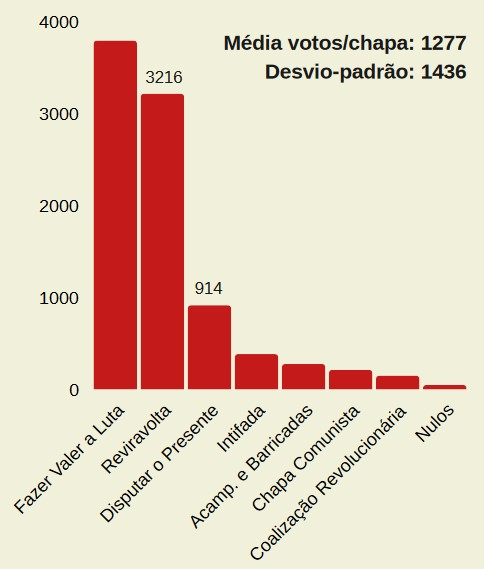
\includegraphics[width=\columnwidth]{textos//img/resultado_geral.jpg}
\end{figure}

Ainda, o resultado das eleições é utilizado na distribuição das cadeiras de representação discente nos órgãos colegiados centrais. A construção da chapa “Unidade Estudantil” é feita proporcionalmente entre as forças políticas concorrentes ao DCE Livre da USP de acordo com os votos totais obtidos na eleição da entidade. 


\subsection*{E a urna do IME?}

A urna do IME contabilizou 209 votos válidos e 1 voto nulo, e os votos ficaram distribuídos da seguinte forma: 

\begin{figure}[H]
    \centering
    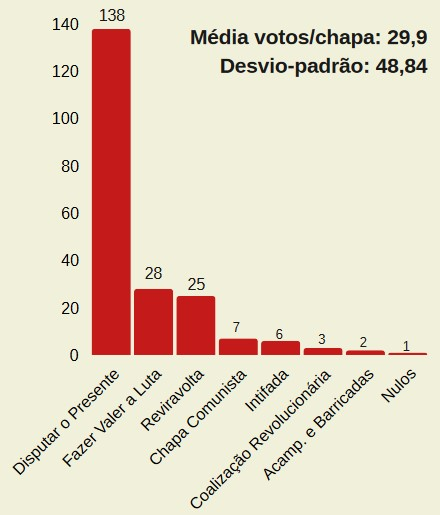
\includegraphics[width=0.88\columnwidth]{textos//img/resultado_ime.jpg}
\end{figure}


\quadradao{\normalsize}{1.2}{0}{\columnwidth}{black}{0.15cm}{
\color{black}
PARA COMPARAR
\\
ELEIÇÕES 2022 - DCE LIVRE DA USP
\\
\raggedright % alinhar à esquerda
\normalfont % para ignorar o bold
Quórum: 10.049
\\~\\
É Tudo Pra Ontem - 6.214\\
Por Todos os Cantos - 1.145\\
Nossa Voz - 1.141\\
USP Sem Medo - 825\\
Envolver - 313\\
Quebra das Correntes - 175\\
Retomada - 87\\
USP Pública, Gratuita e Para Todos - 61\\
Lula Presidente - 47\\
Nulos - 41\\
}

% "EFEITOS DA REDUÇÃO DA JORNADA DE TRABALHO SOBRE OS SALÁRIOS"
\section*{Efeitos da redução da jornada de trabalho sobre os salários}
\autoria{Karl Marx}

[...]

 Todos vocês conhecem a Lei das Dez Horas ou, mais precisamente, das Dez Horas e Meia, promulgada em 1848 [na Inglaterra]. Foi uma das maiores modificações econômicas que já presenciamos. Representou um aumento súbito e obrigatório de salários não em umas poucas indústrias locais, mas nos ramos industriais mais eminentes, aqueles por meio dos quais a Inglaterra domina os mercados do mundo. Foi uma alta de salários em circunstâncias singularmente desfavoráveis. O dr. Ure, o prof. Senior e todos os demais porta-vozes oficiais da burguesia no campo da economia demonstraram (e devo dizer, com razões muito mais sólidas do que as do nosso amigo Weston), que aquilo seria o “dobre de finados” [o ato de soar os sinos pela morte de alguém] da indústria inglesa. Demonstraram que não se tratava de um simples aumento de salário, mas de um aumento de salários provocado pela redução da quantidade de trabalho empregado, e nela fundamentado. Afirmaram que a décima segunda hora que se queria arrancar dos capitalistas era justamente aquela na qual eles obtinham o seu lucro. Ameaçaram com o decréscimo da acumulação, a alta dos preços, a perda dos mercados, a redução da produção, a consequente reação sobre os salários e, enfim, a ruína. Sustentavam que a lei de Maximilian Robespierre sobre os limites máximos [dos preços de mercadorias e salários] era uma ninharia comparada com esta outra; e, até certo ponto, tinham razão. Mas qual foi, na realidade, o resultado?

Os salários em dinheiro dos operários fabris aumentaram, apesar de haver reduzido a jornada de trabalho; cresceu consideravelmente o número de operários em atividade nas fábricas; baixaram constantemente os preços dos seus produtos; desenvolveram-se às mil maravilhas as forças produtivas do seu trabalho e se expandiram progressivamente, em proporções nunca vistas, os mercados para os seus artigos. Em Manchester, na assembleia da Sociedade Pelo Progresso da Ciência, em 1860, eu próprio ouvi o sr. Newman confessar que ele, o dr. Ure, Senior e todos os demais representantes oficiais da ciência econômica se haviam equivocado, ao passo que o instinto do povo não falhara. Cito neste passo o sr. W. Newman e não o prof. Francis Newman, porque ele ocupa na ciência econômica um lugar proeminente, como colaborador e editor da “História dos Preços”, da autoria do sr. Thomas Tooke, essa obra magnífica, que remonta a história dos preços desde 1793 a 1856. Se estive correta a ideia fixa de nosso amigo Weston sobre o volume fixo dos salários de um volume de produção fixo, de um grau fixo de produtividade do trabalho, de uma vontade fixa o constante dos capitalistas e tudo o mais que há de fixo e imutável em Weston, então o prof. Senior teria acertado em seus sombrios presságios, e Robert Owen teria se equivocado, ele que, já em 1816, pedia uma limitação geral da jornada de trabalho como primeiro passo preparatório para a emancipação da classe operária, implantando-a efetivamente, por conta e risco próprios, na sua fábrica têxtil de New Nanark, contra o preconceito generalizados.

[...]

\barraVermelha % uma divisória vermelha

\pagebreak

%%%%%%%%%%%%%%%%%%%%%%%%%%%%%%%%%%%%%%%%%%%%%%%%%%%%%%%%%%%%%%%%%%%%%%
% TESTANDO

\section*{Acontecimentos no CRUSP}
{\color{vermelho_camat} \textbf{Nota conjunta sobre a situação do CRUSP}}
\autoria{14 de agosto de 2024 \\Centro Acadêmico da Matemática, Estatística e\\Computação\\Centro Acadêmico da Física\\Centro Acadêmico Favo 22}


Pela manhã desta quarta-feira (14/08), houveram tensionamentos nos blocos F e G do CRUSP, após a Pró-Reitoria de Inclusão e Pertencimento (PRIP) dar início ao processo de instalação de grades, cujo amplo anúncio havia sido realizado por volta das 7h de hoje (14/08). Vale ressaltar que nesta manhã também estava ocorrendo o ato pelo Dia Nacional dos Estudantes, na Avenida Paulista, não sendo coincidência o início desse processo logo no dia e hora em que parcela dos estudantes mobilizados estariam afastados da universidade.

Dois membros do CAMat estiveram no local, e relatam que a maior parte dos tensionamentos ocorreram no bloco G, onde as instalações estavam mais avançadas, sendo palco para embate entre moradores favoráveis às grades (ligados a gestão anterior da AMORCRUSP) e moradores contrários às grades, ainda que favoráveis a aprimoração de medidas de segurança no CRUSP. As instalações, em ambos os blocos, foram suspensas por hoje após negociação da AMORCRUSP com uma representante da PRIP. Ainda, a associação convoca os moradores para uma assembleia extraordinária, às 17h, para debater os próximos passos frente a essa ofensiva, e endossamos o chamado a todos estudantes do IF, IME e CM e moradores do CRUSP!

Em nota, PRIP publicou um vídeo pelo Instagram colocando a instalação das grades como uma demanda histórica dos moradores, alegando AMORCRUSP (Associação de Moradores do CRUSP) de espalhar desinformação quanto à legitimidade e aprovação dos moradores da medida, uma vez que a instalação foi debatida “com presença da representação estudantil, reunindo quase uma centena de pessoas”. Importante notar a semelhança desses espaços com as audiências sobre a reformulação do PAPFE (vide BoletIME \#3), em que aos estudantes foi dado o poder da voz, mas não o poder de votar e definir concretamente os rumos da política de permanência.

Os CAs signatários entendem que se trata de um assunto delicado e polêmico, dividindo opiniões entre os próprios moradores, sendo um assunto com particularidades e nuances. O CRUSP não é isento de problemas de segurança. De fato, são muitos, e nisso, é necessário compreender que ser contra a instalação de portões e grades não é sinônimo de ser contra um espaço seguro de moradia, como a PRIP insinua dizendo: “A quem interessa ir contra a segurança no CRUSP?”. Ainda, é importante colocar que portões não resolvem os problemas de segurança pela causa, que é um debate necessário e importante, e igualar essas medidas de controle de acesso com segurança da moradia estudantil é contornar esse debate, retirando o cerne político e rebaixando a um debate técnico.

Por isso, reforçamos novamente o chamado aos moradores para comparecerem na assembleia, às 17h30min, e estendemos o chamado para todos estudantes se apropriarem do que vem acontecendo, formulando em conjunto e atuando ativamente, em conjunto dos moradores, nessa luta por moradia digna e segura!

\quadradao{\normalsize}{1.2}{0}{\columnwidth}{black}{0.15cm}{
{\Large Participe ativamente da construção de um CRUSP popular!}
\\~\\
\color{black} \justifying \normalfont % para ignorar o bold
A fim de organizar aqueles interessados em compor a luta por um CRUSP melhor e popular, foi feito o formulário abaixo com objetivo de reunir moradores e simpatizantes que desejam participar ativamente dessa luta.
\\~\\
Queremos construir um espaço de moradia que seja seguro e inclusivo, onde as políticas de segurança sejam formuladas em conjunto com os estudantes que aqui residem.
\\
\begin{figure}[H]
    \centering
    
\includegraphics[width=3cm]{textos//img/crusp_qr_code.png}
    \href{https://forms.gle/8vkN32mbbG5rP9q4A}{https://forms.gle/8vkN32mbbG5rP9q4A}
\end{figure}
}


%%%%%%%%%%%%%%%%%%%%%%%%%%%%%%%%%%%%%%
% Fim da quebra em duas colunas
%%%%%%%%%%%%%%%%%%%%%%%%%%%%%%%%%%%%%%
\end{multicols*}

\pagebreak % quebra de página



%%%%%%%%%%%%%%%%%%%%%%%%%%%%%%%%%%%%%%%%%%%%%%%%%%%%%%%%%%%%%%%%%%%%%%
% TESTANDO

\begin{adjustwidth}{2cm}{2cm}

{\centering \section*{Recado dos editores}}

Car@s leitor@s,

Neste ano de 2024, comemoramos o um ano de aniversário da volta do projeto BoletIME! Em meio ao estresse acadêmico, caos do mundano e preocupações, foi gratificante mais uma vez fazer parte na construção deste espaço de registro e política. O contínuo suporte deste projeto por vocês nos dá a confiança de que estamos trilhando o caminho correto. Por isso, nesta última edição de 2024, nós, do corpo editorial, viemos agradecer por mais um ano de apoio lendo, divulgando e escrevendo para nós. Cada contribuição possui seu valor inquantificável, e disso somos felizes em fazer parte.

Continuaremos aprimorando esse projeto tão gratificante em 2025. Nisso, contaremos e abraçaremos mais uma vez a participação e colaboração de cada um de vocês, leitor@s do BoletIME!

Desejamos um ótimo final de ano, com muitas festas e descanso!

Atenciosamente,\\
Corpo editorial do BoletIME

\vspace{1cm}

\begin{figure}[h]
    \centering
    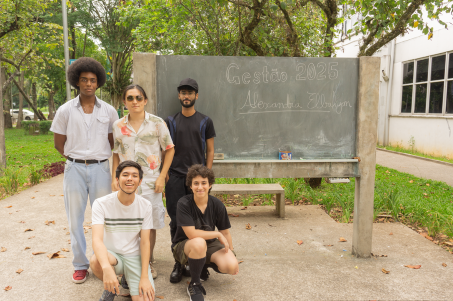
\includegraphics[width=0.6\linewidth]{textos//img/gestao_2025.png}
    \legendaFigura{1.2}{\textit{
    Foto com alguns membros da gestão Alexandra Elbakyan 2025
    \legendaFiguraQuebraLinha
    Em pé, da esquerda para direita: Otávio Fonseca, Link Zhang, Gabriel Marques
    \legendaFiguraQuebraLinha
    Agachado, da esquerda para direita: Eduardo Yukio, Nicolas Miguel
    }}
\end{figure}

\end{adjustwidth}
\pagebreak

%%%%%%%%%%%%%%%%%%%%%%%%%%%%%%%%%%%%%%%%%%%%%%%%%%%%%%%%%%%%%%%%%%%%%%
% TESTANDO
{\centering 

\section*{RETROSPECTIVA CINIME 2024}
\subsection*{\color{black} FILMES POR GÊNERO}

\begin{figure}[H]
    \centering
    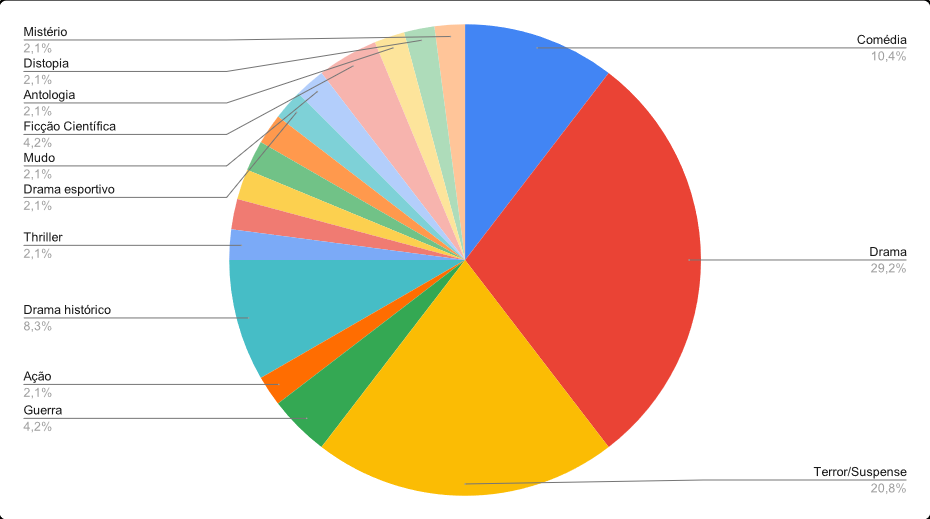
\includegraphics[width=0.95\linewidth]{textos//img/grafico_cinime.png}
\end{figure}
}

\vspace{0.8cm}

\begin{multicols}{2}

    {\centering 
    \subsection*{\color{black} FILMES POR NACIONALIDADE}
    \vspace{.8cm}
    \begin{figure}[H]
        \centering
        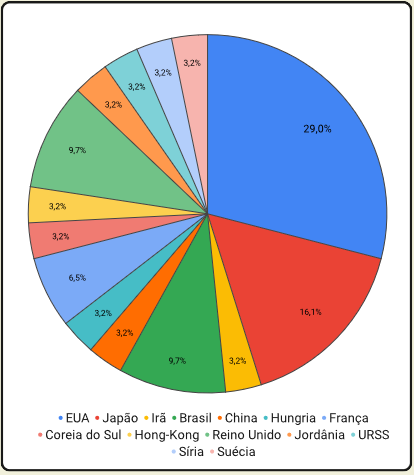
\includegraphics[width=0.9\linewidth]{textos//img/filmes_por_nacionalidade.png}
    \end{figure}
    }

    \subsection*{\color{black} MOSTRAS MENSAIS}
    \textbf{ABRIL: “Propaganda” + evento com CA Panthalassa} \vspace{-0.5cm}
    \begin{itemize}[itemsep=-0.5cm]
        \item Os 800 (2020)
        \item The Red Army/PFLP: Declaration of World War (1971)
        \item O Quinto Selo (1976)
        \item La Chinoise (1967)
    \end{itemize}
    
    \textbf{MAIO: “Coração Vermelho” + Debate “São Paulo, cidade hostil”}\vspace{-0.5cm}
    \begin{itemize}[itemsep=-0.5cm]
        \item Parasita (2019)
        \item Hiroshima, Meu Amor (1959)
        \item Infiltrado na Klan (2018)
        \item São Paulo S/A (1965)
    \end{itemize}

    \textbf{AGOSTO - “Olímpico”}\vspace{-0.5cm}
    \begin{itemize}[itemsep=-0.5cm]
        \item The Duellists (1977)
        \item Farha (2021)
        \item Creed (2015)
    \end{itemize}

\end{multicols}

%%%%%%%%%%%%%%%%%%%%%%%%%%%%%%%%%%%%%%
% Fim do documento
%%%%%%%%%%%%%%%%%%%%%%%%%%%%%%%%%%%%%%
\end{document}
